
\subsection{Introducción teórica}


El objetivo de esta sección es comparar el comportamiento de dos amplificadores operacionales diferentes, analizando sus caracteírsticas principales, contrastando sus respectivos modelos teóricos, simulaciones y mediciones.

En la siguiente tabla se presentan algunas características otorgadas por los fabricantes sobre ambos integrados que serán de importancia en el  análisis que sigue:

%%%Esta tabla esta rota

\begin{table}[H]
\begin{center}
\begin{tabular}{|c|c|c|c|c|c|c|}
\hline
Amplificador   & $A_{vol}$ (dB)   & GBP (MHz)   & Slew Rate (\frac{V}{\mu s})   & V offset (mV)  & I bias (nA)  & $r_d$ %k\Omega \\ \hline
LM833 &  $110$ & $10-15$ & $7$   & $0,3$  & $300$ & no especifica \\ \hline
NE5534 & $25-100$    & $10$  & $7.5$   & $0,5-4$  & $500-1500$&  $100k\Omega$
\\ \hline
\end{tabular}
\caption{Datos op-amps}
\label{tabla:caracteristicas_amps}
\end{center}
\end{table}

El circuito a trabajar es la configuración no inversora dada en la figura \ref{fig:consigna}, en la cual $R_1 = 3k \Omega$, $R_2 = 240k \Omega$ y $R_3 = 220k \Omega$. Se utilizó esta misma configuración para ambos integrados.  


\begin{figure}[H]	
	\centering
	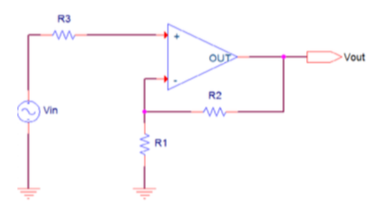
\includegraphics[width=\textwidth]{Ejercicio2/Imagenes/circuito_consigna.png}
	\caption{Configuración no inversora}
	\label{fig:consigna}
\end{figure}

\subsubsection{Respuesta en frecuencia}

Un amplificadores operacional puede describrise mediante diferentes modelos. Un análisis inicial fue hecho en la sección anterior, no obstante aquí se profundizará más al respecto. Un esquema de la configuración no inversora completa puede verse en la figura \ref{fig:esquema_no_inversor}. 

\begin{figure}[H]	
	\centering
	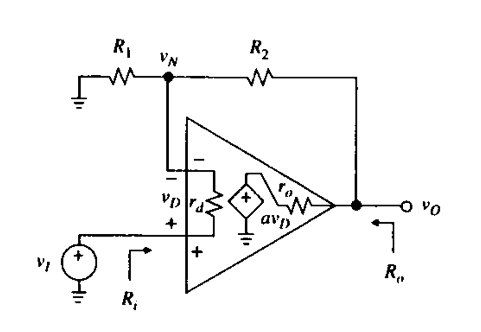
\includegraphics[width=\textwidth]{Ejercicio2/Imagenes/Rin_no_inversor.png}
	\caption{Esquema configuración no inversora completa}
	\label{fig:esquema_no_inversor}
\end{figure}

Para el modelo ideal la resistencia $r_d$ es igual a infinito, mientras que $r_0$ es igual a cero y la ganancia es por ende, infinita. No obstante el caso analizado y medido dista mucho del ideal. En realidad se puede considerar a $A_0$ como un número muy grande, pero finito, al igual que $r_d$. En ese caso se considera que casi no circula corriente por $r_d$ y por ende la tension en el nodo N ($v_N$), es igual a $V_in$. La tension a la salida es a su vez:

\begin{equation}\label{eq:ganancia}
V_{out} = A_{vol}(v_D)
\end{equation}

con $v_D$ igual a la diferencia de tension entre el borne positivo y el negativo. 

Es posible también, realizar un divisor resistivo entre $R_2$ y $R_1$:

\begin{equation}
V_N = \frac{V_{out}R_1}{R_1 + R_2}
\end{equation}

Reemplazando en \ref{eq:ganancia}:

\begin{equation}
V_{out} = A_{vol}(V_{in} - \frac{V_{out}R_1}{R_1 + R_2})
\end{equation}

Si resuelvo para $\frac{V_{out}}{V_{in}}$ y reordeno:

\begin{equation}\label{eq:transferencia_real}
\frac{V_{out}}{V_{in}} = \frac{A_{vol}}{1 + \frac{A_{vol}}{1 + \frac{R_2}{R_1}}}
\end{equation}

Cuando se realiza el límite de $A_vol$ tendiendo a infinito se llega a la expresión ideal:

\begin{equation}\label{eq:ganancia_ideal}
G_i = 1 + \frac{R_2}{R_1}
\end{equation}

El último modelo utilizado es el del polo dominante o compensación por frecuencia. Debido a que la mayoría de los amplificadores utilizan el feedback negativo como método para alcanzar altas ganancias, es posible que a altas frecuencias, imperfecciones dentro del chip generen que este feedback se de vuelta, causado que elamplificador oscile. 

%%Se puede incluir mñas teoría sobre compensación de polos

El modelo de polo dominante utilizado es el siguiente:

\begin{equation}\label{eq:polo_dominante}
A_{vol} = \frac{A_0}{1 + \frac{s}{\omega_p}}
\end{equation}

en el cual $\omega_p$ es del orden de los Herzs.
Si se reemplaza \ref{eq:polo_dominante} y \ref{eq:ganancia_ideal} en \ref{eq:transferencia_real}, con un poco de trabajo matemático se llega a la siguiente fórmula normalizada:

\begin{equation}\label{eq:ganancia_completa_normalizada}
\frac{V_{out}}{V_{in}} = \frac{\frac{G_iA_0}{A_0 + G_i}}{1 + \frac{s}{\omega_p(1 + \frac{A_0}{G_i})}}
\end{equation}

Por último, un parámetro de vital importancia para el análsis de un amplificador operacional es su GBP, o el producto entre el ancho de banda del amplificador y la gananci a la cual es medido. Para cualquier op-amp con polo dominante esta cantidad es una constante independiente de la ganancia a la cual es medida. El gain-bandwidth product, es importante ya que, da una idea de la máxima ganancia que se puede extraer de un dispositivo a una frecuencia dada. El GBP para un amplificador operacional con polo dominante es igual a la siguiente expresión:

\begin{equation}\label{eq:GBP}
GBP = A_0\omega_p = G_{real}\omega_c
\end{equation}

con $\omega_c$ el polo del circuito completo.


\subsubsection{Impedancia de entrada}

Para analizar la impedancia de entrada teórica del circuito se utilizó el modelo completo con polo sominante del op-amp. Todo el análisis siguiente se hará a partir de la figura \ref{fig:esquema_no_inversor}, con la única diferencia de que se considerará además una resistencia en la entrada no inversora del circuito ($R_3$). La impedancia de entrada del circuito puede obtenerse poniendo una fuente de prueba $v$ a la entrada del circuito para luego usar la relación:

\begin{equation}\label{eq:zin}
Z_{in} = \frac{v}{i}
\end{equation}

En primer lugar se plantea la ecuación de corrientes en el nodo N:

\begin{equation}\label{eq:corrientes_N}
\frac{v - v_N}{R_3 + r_d} - \frac{v_N}{R_1} + \frac{A_{vol}v_D - v_N}{R_2} = 0
\end{equation}

Se por inspección que:

\begin{equation}\label{eq:v_N}
v - v_D = v_N = v - r_di
\end{equation}

Reemplazando \ref{eq:v_N} en \ref{eq:corrientes_N} y simplificando:

\begin{equation}
\frac{r_di}{R_3 + r_d} - \frac{v}{R_1} + \frac{r_di}{R_1} +\frac{A_{vol}r_di - v + r_di}{r_0 + R_2} = 0
\end{equation}

Si se factoriza la expresión anterior de un lado por i y del otro por v:

\begin{equation}
i(\frac{r_d}{r_d + R3} + \frac{r_d}{R_1} + \frac{A_{vol}r_d}{r_0 + R_2}) = v(\frac{1}{R_1} + \frac{1}{r_0 + R_2})
\end{equation}

Si se reemplaza \ref{eq:zin} en la ecuación anterior se cancelan las corrientes. Luego resuelvo para $Z_i$ y después de reordenar la expresión resultante es la siguiente:

\begin{equation}\label{eq:zin_real}
Z_i = r_d(\frac{R_1 // (r_0 + R_2)}{r_d + R_3} + 1 + \frac{A_{vol}}{1 + \frac{r_0 + R_2}{R_1})})
\end{equation}

Si se reemplaza $A_{vol}$ por su modelo de polo dominante y se reordena se llega a lo siguiente:

\begin{equation}\label{eq:zin_completa}
Z_i = r_d(1 + \frac{R_1 // (r_0 + R_2)}{r_d + R_3} + \frac{\frac{A_0}{1 + \frac{r_0 + R_2}{R_1}}}{1 + \frac{s}{\omega_p}}
\end{equation}

Por último es importante mencionar el método de medición de $Z_i$. Para eso se modeló el circuito como si fuera un divisor resistivo, es decir, se colocó una resistencia extra de $1k\Omega$ a la entrada del circuito y se midió cuanta tensión caía sobre dicha resistencia con el osciloscopio. Se hizo lo mismo para la fase, aunque los resultados finales pueden mejorarse. 


\subsection{Resultados experimentales LM833}

Con los valores de resistencias utilizados la ganancia ideal tiene un valor de 81, \ref{eq:ganancia_ideal}, valor a tener en cuenta a la hora de medir, para evitar tener problemas con el slew rate o que el amplificador sature. Por lo anterior se utilizaron tensiones del orden de los milivoltios para medir la respuesta en frecuencia. De \ref{eq:GBP}, considerando el peor caso para el GBP brindado por el fabricante $(10 Mhz)$, se obtiene que:

\begin{equation}\label{eq:frecuencia_corte_LM833}
f_c = \frac{GBP}{2\pi G_i} = 19649 Hz
\end{equation} 

Se toma $G_i$ ya que $A_0$ es considerablemente grande y por ende $G_i$ es cercano a $G_{real}$. 


Por último antes de pasar al análisis de la respuesta en frecuencia del circuito con el LM833, al realizarse las mediciones se observó que a medida que la frecuencia de la señal de entrada aumentaba aparecía un offset en la señal de salida. En otras palabras, había una componente de continua montada sobre la señal de salida, por ende el valor medio de la salida es diferente a $0 V$. A pesar de lo anterior, este fenómeno solo se pudo apreciar a frecuencias relativimante altas (orden de los Megahertz). Debido a que el LM833 tiene una impedancia entre sus bornes muy grande (orden de los Megaohm), a frecuencias bajas no se observa un offset en la salida. Pero a medida que la frecuencia aumenta, a su vez disminuye la impedancia de entrada del circuito y así, se hace comparable el valor de $R_3$ con el de $Z_i$. Lo anterior ocasiona que haya una corriente entrando al amplificador, llámese Input Bias Current, que haya una caída de tensión no deseada a la entrada y se degrade la condicón de Tierra virtual. 

\subsubsection{Respuesta en frecuencia}

Ya habiendo descrito los modelos teóricos y su respectivo método de medición, se procede a presentar los gráficos obtenidos en los cuales se superpone el modelo teórico, las simualciones realizadas en LTSpice y los datos medidos:



\begin{figure}[H]	
	\centering
	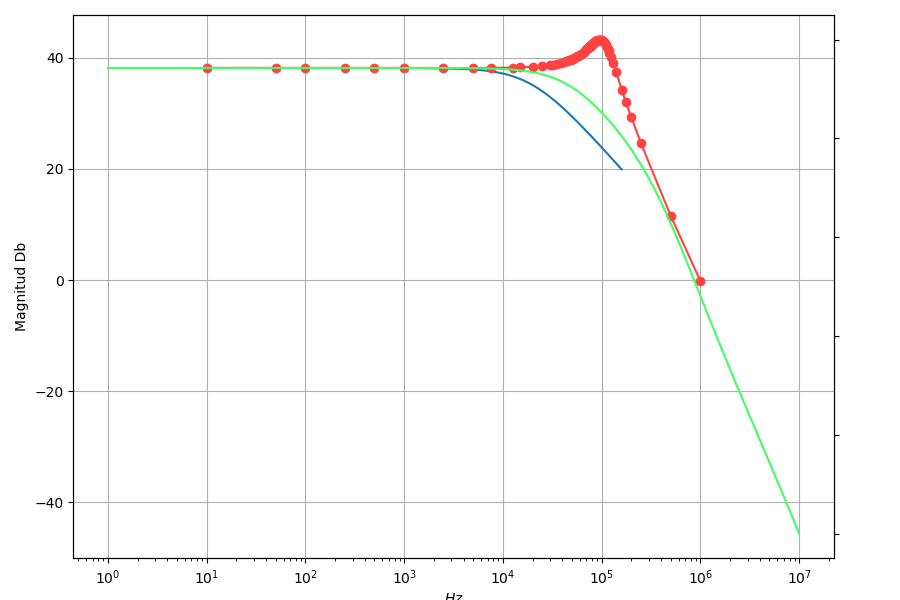
\includegraphics[width=\textwidth]{Ejercicio2/Imagenes/Bode_Amp_LM833.png}
	\caption{Diagram de Bode en amplitud para LM833}
	\label{fig:bode_amp_LM833}
\end{figure}

\begin{figure}[H]	
	\centering
	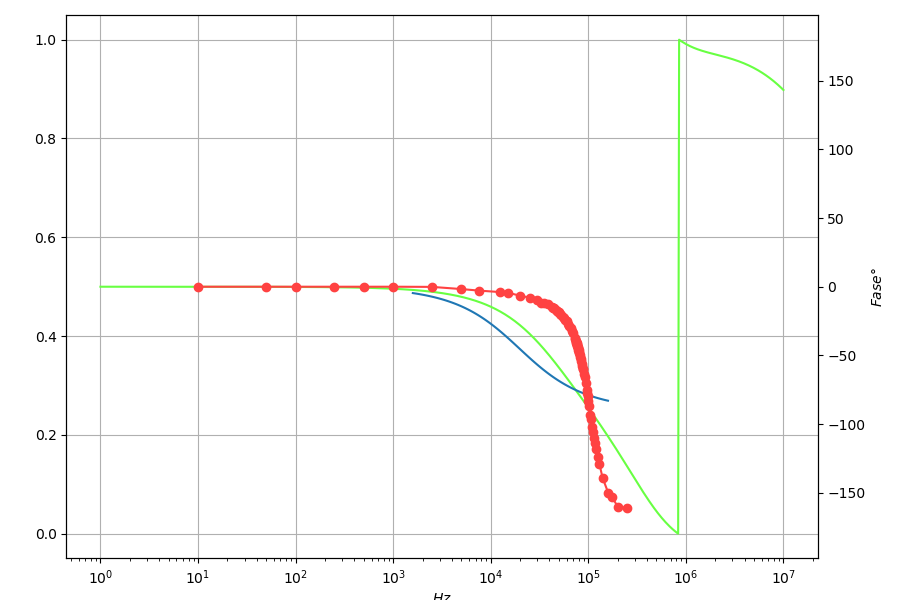
\includegraphics[width=\textwidth]{Ejercicio2/Imagenes/Bode_Fase_LM833.png}
	\caption{Diagram de Bode en fase para LM833}
	\label{fig:bode_fase_LM833}
\end{figure}

%%NO salieron colores, agregar despues


En primer lugar puede verse en el gráfico \ref{fig:bode_amp_LM833} que la frecuencia de corte obtenida en \ref{eq:frecuencia_corte_LM833} concuerda con el modelo simulado. Lo que no concuerda con el modelo simualdo y menos aún con el teórico es el sobrepico medido. El resultado esperado era un circuito que se asemeje a un pasa-bajos de primer orden, no obstante el sobrepico indica que el circuito real obedece a un modelo de segundo orden. Se pueden buscar razones para explicar este resultado. Por el solo acto de medir se esta agregando una capacitancia de $11pF$ debido a las puntas, además se tiene que tener en cuenta la capacitancia de las patas de los componentes y que el circuito fue medido en un protoboard, el cual agrega aproximadamente $2pF$ por cada conexión hecha. El pico observado en un principio fue un problema para las mediciones, ya que el amplificador llegaba a su punto de saturación cerca del máximo. Más allá de esta anomalía el resto del gráfico es acorde a las simulaciones y la teoría. 

Por otro lado puede hacerse el mismo análisis con la fase del circuito. Teoricamente uno esperaría medir un circuito de primer orden, en el cual es desfase máximo es de 90 grados, pero las evidencias empíricas demuestran lo contrario, se esta trabajando con un circuito de segundo orden y un desfase de 180 grados. Incluso puede observarse a que a altas frecuencias hay un salto en la fase simulada, comportamiento que no logró medirse en el laboratorio.

Un primer paso para mejorar las mediciones es realizar el circuito en una PCB y asi disminuir las capacidades parásitas. Agregado a lo anterior, una solución al problema de las capacidades parásitas es incluir algún tipo de circuito de compensación, similar a lo que hacen los fabricantes al agregar un capacitor dentro del op-amp para evitar la inversión del feedback. El fabricante no incluyó ningún tipo de circuito de compensación recomendado en el caso del LM833 

\subsubsection{Impedancia de entrada}

Para graficar la impedancia de entrada teórica hacen falta datos respecto de las resistencias internas del aplificador que no fueron dados por el fabricante. Para poder tener una comparación con los datos medidos, se propone una $r_d = 2,5M\Omega$ y una $r_0 = 20 \Omega$. 

%%bode impedancia entrada LM833

Es importante destacar que a frecuencias menores a los $100 Hz$ fue imposible la medir una caida de tension en la resistencia colocada en serie delante del circuito. Es importante observar la expresion obtenida en \ref{eq:zin_completa} y ver como se comporta a medida que varía la frecuencia. A frecuencias bajas la resistencia tiende $r_d$, es decir un valor muy grande, razón por la cual fue imposible medir caidas de tensión. Luego lo esperado es que el modulo de la impedancia baje hasta llegar a un valor constante, comportamiento que se evidencia en los gráficos anteriores.  


\subsection{Resultados experimentales NE5534}

Debido a que el dato de GBP dado por el fabricante es el mismo que el valor mínimo para el amplificador anterior la frecuencia de corte del circuito teórica será aproximadamente la misma, considerando que se tiene la misma ganancia ideal. No obstante lo anterior, el NE5534 posee un $A_{vol}$ con muchísima disperisón, por lo que se tomó el valor típico del mismo. Además la resistencia de entrada en este caso es mucho menor, igual a $100k\Omega$ en el mejor de los casos. Debido a esto, cuando se comenzó a medir con $R_3 = 220k\Omega$ no se logró que el circuito funcionara. Como $R_3$ era del mismo orden, en este caso mayor, que $R_{in}$ el circuito funcionaba como un divisor resistivo que además amplificada el ruido que entraba al sistema. En la figura siguiente se ve el efecto medido en un principio:


\begin{figure}[H]	
	\centering
	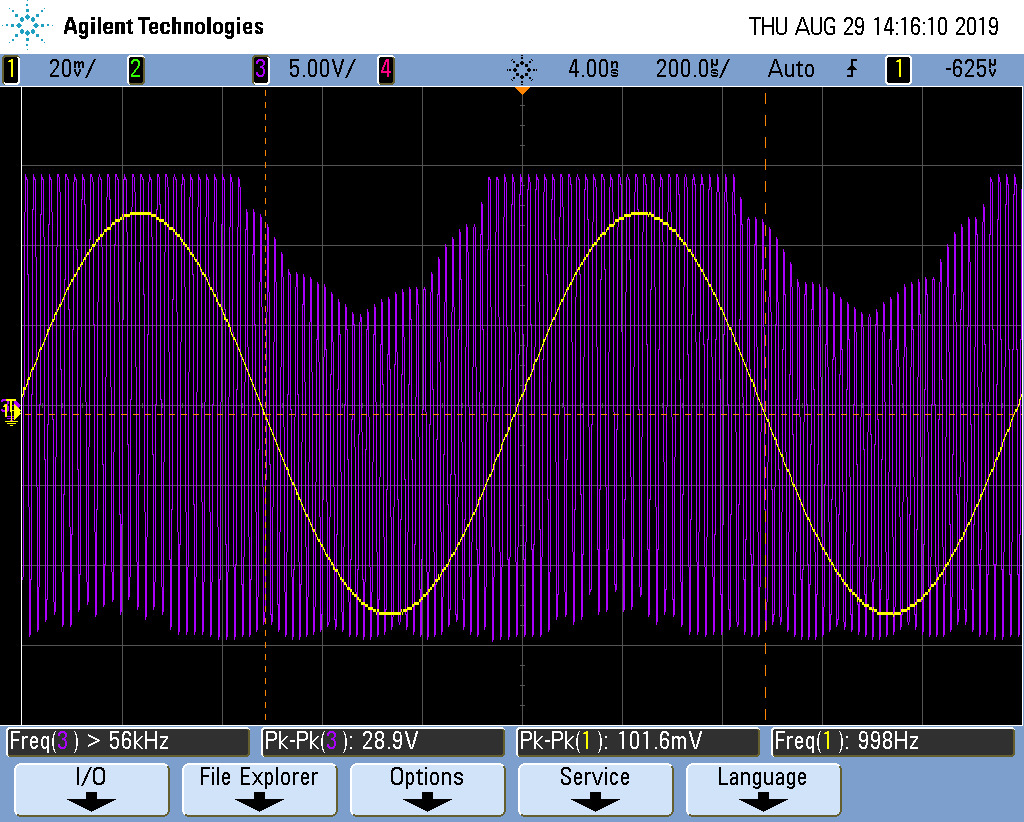
\includegraphics[width=\textwidth]{Ejercicio2/Imagenes/ruido.png}
	\caption{Ruido medido en NE5534}
	\label{fig:ruido}
\end{figure}

Para evitar lo anterior, se reemplazó la resistencia $R_3$ por una igual a $22k\Omega$. El segundo efecto visto fue el de un offset en la señal de salida. Para este operacionale el offset sí podía apreciarse a bajas frecuencias y era muy notorio a medida que éstas aumentaban. Para evitar lo anterior el fabricante ofrece un circuito de compensación en su datasheet, en el cual se le agrega un capacitor adicional al circuito. A pesar de eso las mediciones fueron realizadas sin el circuito de compensación.

\subsubsection{Respuesta en frecuencia}
Los resultados obtenidos se presentan en los gráficos a continuación:

\begin{figure}[H]	
	\centering
	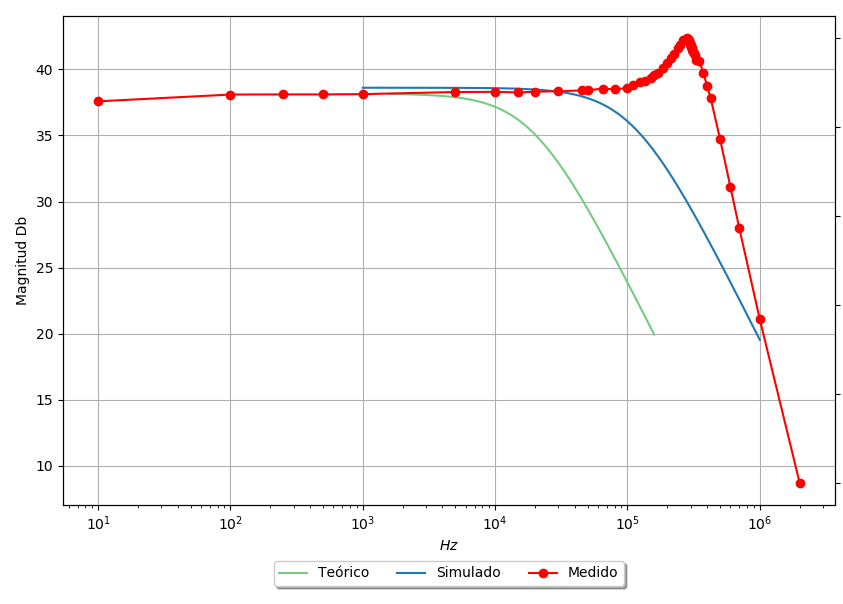
\includegraphics[width=\textwidth]{Ejercicio2/Imagenes/Bode_Amp_NE5534.png}
	\caption{Diagrama de Bode en amplitud para NE5534}
	\label{fig:bode_amp_NE5534}
\end{figure}

\begin{figure}[H]	
	\centering
	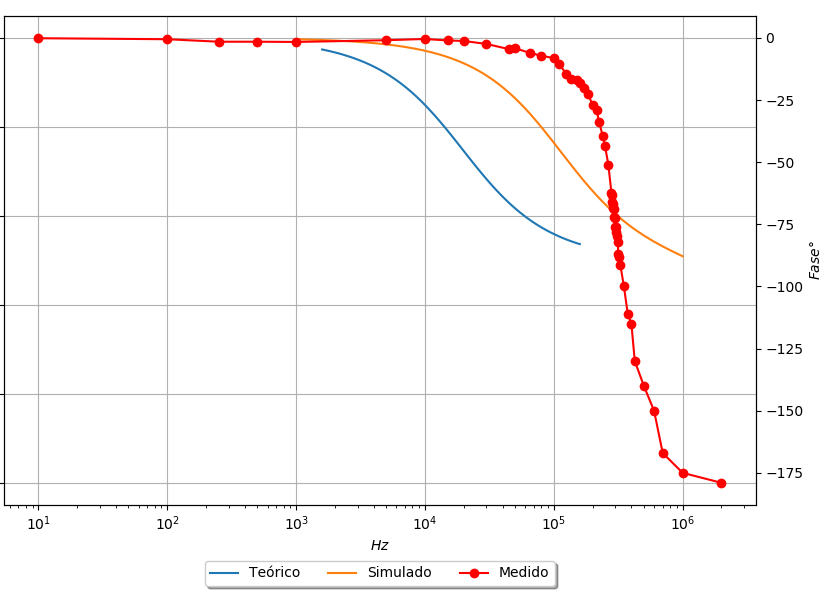
\includegraphics[width=\textwidth]{Ejercicio2/Imagenes/Bode_Fase_NE5534.png}
	\caption{Diagrama de Bode en fase para NE5534}
	\label{fig:bode_amp_NE5534}
\end{figure}

Al igual que en el amplificador anterior, se midió un sobrepico cercano a la frecuencia de corte del circuito. En este caso, dicho sobrepico es aún mayor que para el LM833, lo que indica mayores capacidades parásitas. Además la frecuencia a la que ocurre dicho sobrepico es mayor a la frecuencia teórica calculada anteriormente. Debido a que la ganancia ideal es igual para ambas configuraciones, la única diferencia está el GBP del integrado. Es fácil ver entonces que la ganancia en dBS para el NE5534 alcanza un sobrepico mayor que el LM833 pero es menor en el segmento en el que es constante. De esta manera queda demostrado el efecto del producto de ancho de banda en un operacional y como varía de modelo en modelo. En el NE5534 se logra un mayor ancho de banda, a cambio de perder un poco de ganancia, mientras que en el LM833 ocurre lo contrario. En ambos gráficos puede verse también que debido a las capacidades parásitas el circuito se comporta como uno de segundo orden experimentalmente.

Además de lo anteriormente descrito las mediciones concuerdan bastante bien con los modelos en las secciones en que son cuasi-lineales en el caos de la amplitud, y se puede observar una tendencia similar en el diagrama de fase, a pesar de haberse medido esencialmente un circuito de segundo orden.

\subsubsection{Impedancia de entrada}
El análisis de la impedancia de entrada para el NE5534 es idéntico al chip anterior, con la salvedad de que si pudieron medirse impedancias a menores frecuencias gracias a que la impedancia de entrada del circuito es muchísimo menor para este operacional. Para realizar estas mediciones tampoco se recurrió al circuito de compensación.

%%Inserto gráficos impedancia de entrada

\subsection{Aplicaciones}
Los dos amplificadores aquí tratados poseen características que los hacen deseables para cierto tipo de aplicaciones. Ambos poseen un $A_{vol}$, y por consiguiente, una ganancia relativamente grande en un ancho de banda amplio. Lo anterior hace que ambos amplificadores sean útiles en aplicaciones de Audio y preamplificación, ya que el rango de frecuencias en el que se manejan concuerda con ese tipo de aplicaciones. Además, el LM833 posee una impedancia de entrada muy grande y una impedancia de salida muy chica, lo que lo convierte en un gran adaptador de impedancias, no así el otro op-amp analizado. Una desventaja del LM833 es que no hay una manera de integrar un circuito de balance al mismo, al contrario que con el NE5534. 


\subsection{Conclusiones}

En el diseño de un circuito hay que tener en cuenta diversos factores a la hora de elegir que elemento utilizar. En el caso de los amplificadores operacionales, no solo importa la ganancia sino que es de vital importancia analizar las impedancias de entrada y de salida. Como ocurrió en el desarrollo de este ejercicio, a la hora de medir dichos parámetros fueron fundamentales a la hora de armar los circuitos deseados. El caso analizado es quizás el más simple de los circuitos, no así el menos importante de comprender. En caso de tener circuitos con diversas fases el no tener en cuenta factores como los nombrados anteriormente puede significar la diferencia entre recibir una señal limpia o medir ruido a la salida de un sistema. Por eso, queda como conclusión final que es deber de cualquier diseñador tener en cuenta la mayor cantidad posible de variables en la implementación de un circuito.